\documentclass[12pt,a4paper]{report}
\usepackage[utf8]{inputenc}
\usepackage{setspace}
\usepackage{titlesec}
\usepackage{fancyhdr} 
\usepackage{lipsum} 
\usepackage{amsmath} % For mathematical formatting
\usepackage{graphicx}
\usepackage{color}
\usepackage{listings}
\usepackage{newtxtext} % Times New Roman for text
\usepackage{newtxmath} % Times New Roman for math
\titleformat{\chapter}[hang]{\bfseries\Large}{\thechapter.}{1em}{}
\titleformat{\section}[hang]{\bfseries\large}{\thesection}{1em}{}
%\usepackage{hyperref}
\usepackage{xcolor, colortbl}
\setlength{\topmargin}{-0.5in}
\setlength{\oddsidemargin}{0.5in}
\setlength{\evensidemargin}{0.5in}
\setlength{\textwidth}{6in}
\setlength{\textheight}{9in}
\setstretch{1.5}
\usepackage{pgfplots}
\usepackage{acronym}
\usepackage{pgfplots}
\pgfplotsset{compat=1.17}

\definecolor{codegray}{rgb}{0.5,0.5,0.5}
\definecolor{codepurple}{rgb}{0.58,0,0.82}
\definecolor{backcolour}{rgb}{0.95,0.95,0.92}
\definecolor{lightblue}{rgb}{0.678, 0.847, 0.902}
\definecolor{lightpink}{rgb}{1.0, 0.71, 0.76}
\definecolor{lightcoral}{rgb}{0.941, 0.502, 0.502}
\definecolor{peachpuff}{rgb}{1.0, 0.99, 0.99}

\lstdefinestyle{mystyle}{
	backgroundcolor=\color{peachpuff},
	commentstyle=\color{codegray},
	keywordstyle=\color{blue},
	numberstyle=\tiny\color{blue},
	stringstyle=\color{codepurple},
	basicstyle=\ttfamily\footnotesize,
	breakatwhitespace=false,
	breaklines=true,
	captionpos=b,
	keepspaces=true,
	numbers=left,
	numbersep=5pt,
	showspaces=false,
	showstringspaces=false,
	showtabs=false,
	tabsize=2
}
\lstset{style=mystyle}

\pagestyle{fancy}
\fancyhf{}
\fancyhead[R]{\thepage}
\fancyfoot{}
\renewcommand{\headrulewidth}{0pt} 

\begin{document}
		





% After the previous pages, set the page number to 1
\setcounter{page}{1}
\pagenumbering{arabic} % Starts page numbering from 1 with Arabic numerals


	\begin{center}
		\textbf{\Large CHAPTER 1}\\[0.5cm]
		\textbf{\Large INTRODUCTION}
	\end{center}
	
\section*{1.1 Introduction}

\hspace{1cm}Tomatoes are a key agricultural product, and their quality significantly impacts consumer satisfaction and market competitiveness. The global demand for high-quality tomatoes has increased, driven by consumers' growing preference for fresh and healthy produce. Traditionally, the grading and sorting of tomatoes have been performed manually. This method, however, is time-consuming, labor-intensive, and prone to human error, leading to higher costs and inefficiencies. In large-scale production environments, where the demand for high-quality produce is constant, manual methods fail to meet rising consumer expectations and global market standards efficiently\cite{ref7}. These inefficiencies often disrupt the supply chain, creating bottlenecks that reduce overall productivity and profitability for producers.Furthermore, as the agricultural sector faces labor shortages and increasing labor costs, there is a pressing need to adopt automation to ensure consistent and reliable quality control. Traditional grading methods also struggle to account for subtle variations in tomato quality, such as size, color, and texture, which are critical for determining ripeness and overall quality. As a result, there is an urgent demand for innovative solutions that can enhance the efficiency, accuracy, and scalability of the tomato grading process.

Recent advances in computer vision and machine learning technologies have shown great potential in automating quality control tasks. These technologies can provide a more precise, consistent, and faster alternative to manual grading, offering the ability to sort tomatoes based on multiple quality factors in real-time. The integration of deep learning models, such as convolutional neural networks (CNNs), with automated systems can significantly improve the grading process, reduce errors, and increase throughput, thereby boosting the profitability and sustainability of tomato production.

	
\section*{1.2 Problem Statement}
\hspace{1cm}Manual grading systems are inadequate for handling the high volume of tomatoes produced daily. These systems result in several inefficiencies, including delays due to increased operational time, higher costs due to greater reliance on labor, and inconsistencies in grading that negatively impact market value and customer satisfaction. These challenges highlight the need for an automated system that can accurately assess tomato quality at scale, reduce labor dependency, and enhance precision and consistency in grading.
	
	\section*{1.3 Objective}
\hspace{1cm}The primary goal of this research is to develop a real-time, automated system for tomato quality grading and sorting. The system aims to efficiently classify tomatoes using both binary classification (healthy vs. rejected) and multiclass classification (ripe, unripe, old, and damaged). Additionally, the system seeks to reduce labor costs, improve operational efficiency, and evaluate its performance using metrics such as accuracy, precision, recall, and F1-score. 

As shown in Figure \ref{fig:tomato_quality_system}, the system provides an overview of the tomato quality grading process.


\begin{figure}[htbp]
	\renewcommand\thefigure{1.1}
	\centering
	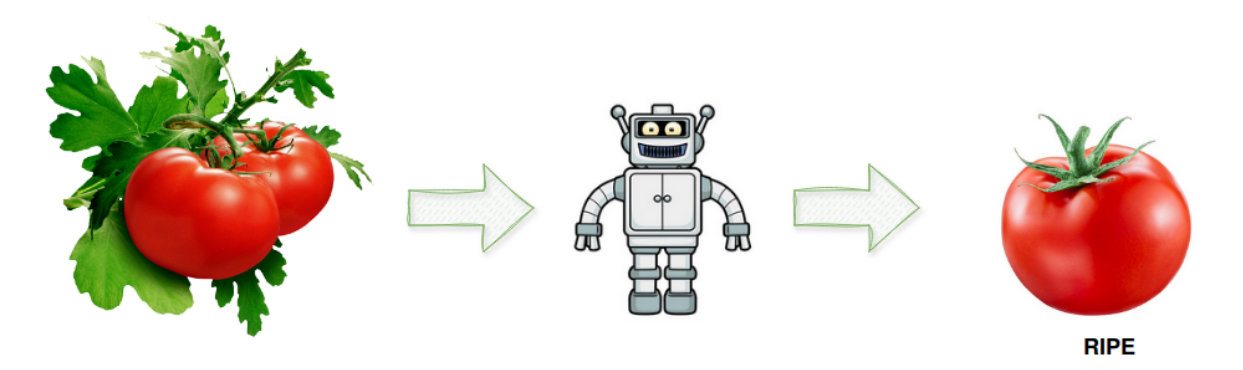
\includegraphics[width=1\textwidth]{DOC/obj.png}
	\caption{Overview of the Tomato Quality Grading System. }
	\label{fig:tomato_quality_system}
\end{figure}


    \section*{1.4 Proposed Solution}
    \hspace{1cm}This research introduces an automated grading system that leverages a hybrid model approach, combining deep learning and traditional machine learning techniques. The system uses pre-trained convolutional neural networks (CNNs) for feature extraction, enabling it to capture complex features from tomato images. These extracted features are classified using machine learning algorithms, including Support Vector Machines (SVM), k-Nearest Neighbors (KNN), and Decision Trees (DT). To ensure practical application and robustness, the system is trained on a custom dataset sourced from field environments. This hybrid approach is designed to address the inefficiencies of manual grading systems and enhance the accuracy and scalability of tomato quality assessment.
	
\section*{1.5 Organization of the Thesis}

\hspace{1cm}The thesis is organized as follows: Chapter 1 introduces the study, including the problem statement, objectives, proposed solution, and organization of the thesis. Chapter 2 reviews the literature, discussing related work and summarizing key findings. Chapter 3 presents the system design, including an overview, dataset description, feature extraction using pre-trained CNNs, classification methods, and performance metrics. Chapter 4 covers the implementation and results, featuring the system architecture, implementation setup, results of feature extraction and classification tasks, evaluation with performance metrics, and a discussion of the findings. Finally, Chapter 5 concludes the study and provides future work.


	
	\newpage
	
	\begin{center}
		\textbf{\Large CHAPTER 2}\\[0.5cm]
		\textbf{\Large LITERATURE REVIEW}
	\end{center}
	
\section*{2.1 Introduction}

\hspace{1cm}\hspace{1cm}Significant advancements have been made in automated systems for sorting and grading fruits and vegetables, focusing on external attributes such as shape, size, color, texture, and ripeness. The increasing demand for high-quality produce and the limitations of manual grading have driven the shift towards automation. Many studies have explored algorithms combining image processing with machine learning and deep learning to improve the accuracy and efficiency of these systems. Traditional machine learning algorithms like support vector machines (SVM), k-nearest neighbors (KNN), and decision trees (DT) have been used, relying on hand-crafted features such as color histograms and texture descriptors. These approaches, while effective to an extent, often struggle to capture the complex, non-linear patterns inherent in real-world data, especially when dealing with natural objects like fruits and vegetables.

The advent of deep learning, particularly convolutional neural networks (CNNs), has significantly improved fruit grading systems by automatically learning hierarchical features from raw image data. This process eliminates the need for manual feature extraction, making it possible to detect subtle patterns that traditional methods might miss. CNNs can capture complex features like edges, textures, and shapes at multiple levels of abstraction, allowing them to classify and grade produce with greater accuracy and efficiency.

Additionally, techniques like transfer learning, data augmentation, and multispectral imaging have further enhanced model performance. Transfer learning enables the reuse of pre-trained models, reducing the need for large amounts of labeled data, which can be difficult to obtain in agricultural applications. Data augmentation artificially increases the size of training datasets by generating variations of existing images, improving model generalization. Multispectral imaging, which captures data beyond the visible spectrum, allows for better evaluation of both external and internal fruit quality attributes such as ripeness, sugar content, and firmness. Despite these advancements, challenges such as handling variations in lighting, background interference, and environmental conditions persist. Ongoing research aims to improve the robustness and scalability of these systems, ensuring their practical application in large-scale agricultural environments.


	\section*{2.2 Related Works}

	\textbf{Real-time Defects Detection System for Orange Citrus Fruits Using Multi-spectral Imaging} \ This study focuses on developing an algorithm for defect identification in oranges using a dual-sensor camera that captures both RGB and near-infrared (NIR) images. The system employs a thresholding approach followed by a voting technique for color combination to detect defects. The algorithm demonstrated a high accuracy of 95\% in defect detection, proving its effectiveness in fruit quality assessment. By combining visible and near-infrared light, the system is capable of detecting not only external surface defects but also internal issues like rot, enhancing the overall fruit evaluation process. The results of this study highlight the potential of multispectral imaging to provide more comprehensive quality assessments, addressing limitations seen in traditional visual inspection methods\cite{ref1}.
	
	\vspace*{0.8cm} \textbf{Hybrid Feature Extraction and Machine Learning Approach for Fruits and Vegetable Classification} \ This study presents a comparative analysis of machine learning algorithms for vegetable and fruit classification. SVM was compared with KNN, with SVM achieving superior accuracy of 94.3\%, indicating its greater suitability for classifying agricultural produce based on visual features. The study explores the importance of selecting the right feature extraction methods, such as color, texture, and shape, and how they can influence the performance of machine learning models. It highlights that while KNN offers simplicity, SVM provides better results, especially when combined with robust feature extraction techniques. This research demonstrates that hybrid approaches, integrating machine learning with image processing, are crucial for enhancing fruit and vegetable classification systems\cite{ref2}.
	
	\vspace*{0.8cm} \textbf{A Hybrid CNN–SVM Classifier for Weed Recognition in Winter Rape Field} \ The study proposed a hybrid model combining VGGNet with Support Vector Machines (SVM) for weed identification in winter rape fields. The hybrid model achieved an accuracy of 92.1\%, showcasing the potential of combining deep learning and machine learning techniques for agricultural applications, particularly in precision farming. This work emphasizes the advantage of using deep learning models like VGGNet for automatic feature extraction, combined with the power of SVM to enhance classification accuracy. The approach offers great promise in automating weed detection, reducing labor costs, and ensuring efficient resource management in farming\cite{ref3}.
	
	\vspace*{0.8cm} \textbf{Classification of Appearance Quality of Red Grapes Based on Transfer Learning of CNNs} \ This study focused on classifying the appearance quality of red grapes using transfer learning with CNNs. The researchers employed pre-trained models like VGG19, VGG16, GoogleNet, and ResNet50, with ResNet50 demonstrating the best performance, achieving 82.85\% accuracy. Combining ResNet50 with SVM further improved the accuracy to 95.08\%, demonstrating the effectiveness of transfer learning in fruit classification. The use of transfer learning allows the model to leverage existing knowledge from large datasets, significantly improving performance, even with limited data from the target domain. This method is particularly useful for fruit quality evaluation, where acquiring labeled data can be time-consuming and costly\cite{ref4}.
	
	\vspace*{0.8cm} \textbf{Tomato Ripeness Detection and Classification Using VGG-based CNN Models} \ This study employed a VGG-based CNN model for tomato ripeness detection and classification. Using transfer learning techniques with VGG-16, the model achieved 96\% accuracy in classifying tomatoes into ripe and unripe categories, highlighting the potential of deep learning for ripeness detection. This research demonstrates the feasibility of applying deep learning in real-time agricultural systems, where the accurate detection of ripeness is crucial for harvesting decisions. The approach offers a reliable, automated solution that can be integrated into larger food sorting and grading systems\cite{ref5}.
	
	\vspace*{0.8cm} \textbf{Size Classification of Tomato Fruit Using Thresholding, Machine Learning, and Deep Learning Techniques} \ This study presented a tomato classification system based on size, utilizing both machine learning (SVM) and deep learning techniques. It classified tomatoes based on features such as area, perimeter, and enclosed circle radius. The SVM achieved 94.5\% accuracy, outperforming other machine learning techniques. The study underlines the importance of incorporating multiple techniques to tackle different challenges in agricultural grading systems. By leveraging both traditional and advanced methods, the system achieves high accuracy while being adaptable to various fruit types and grading requirements\cite{ref6}.
	
	\section*{2.3 Summary}
\hspace{1cm}In summary, various automated systems have been developed for fruit and vegetable quality assessment, leveraging different algorithms and techniques. The combination of image processing, machine learning, and deep learning has shown promising results in tasks such as defect detection, classification of ripeness, and size classification. Studies have demonstrated the effectiveness of methods such as transfer learning, SVM, and CNN-based models in achieving high accuracy rates for various agricultural applications. Additionally, hybrid approaches that combine traditional machine learning techniques with deep learning models, such as CNN–SVM, have proven to be particularly effective, achieving better performance than standalone models.

The application of transfer learning, especially with pre-trained CNNs like VGG, ResNet, and GoogleNet, has enabled researchers to tackle complex classification tasks with limited training data. This has proven beneficial in agricultural settings where large labeled datasets are often scarce. Furthermore, multispectral and near-infrared imaging techniques have emerged as valuable tools for providing additional insights into the internal quality of fruits, complementing traditional visual inspection methods.

However, despite these advancements, several challenges remain. Variability in environmental conditions, such as lighting and background noise, continues to affect the accuracy and reliability of these automated systems. Researchers are actively working on improving the robustness of models to handle these challenges, aiming for scalability and consistency across different agricultural environments. Future advancements in hardware, such as more sophisticated multispectral cameras, and the development of more efficient algorithms will likely contribute to overcoming these limitations. As the technology continues to evolve, it holds great potential for revolutionizing the agricultural industry by enabling more efficient and accurate grading systems that can be deployed on a large scale.

	
		\newpage
	
	\begin{center}
		\textbf{\Large CHAPTER 3}\\[0.5cm]
		\textbf{\Large SYSTEM DESIGN}
	\end{center}
	\section*{3.1 Proposed System Overview}
\hspace{1cm}The proposed system is a real-time, automated tomato quality grading and sorting system that utilizes deep learning and traditional machine learning models, as shown in Figure \ref{fig:proposed_system}. The system classifies tomatoes for both binary (healthy vs. rejected) and multiclass (ripe, unripe, old, and damaged) tasks. It leverages pre-trained Convolutional Neural Networks (CNNs) for feature extraction, followed by traditional classifiers like Support Vector Machines (SVM), k-Nearest Neighbors (kNN), and Decision Trees (DT) for classification. Data augmentation techniques such as rotation, flipping, brightness adjustments, and noise addition enhance the model's generalization. The system is designed to reduce labor costs, improve operational efficiency, and deliver high accuracy, precision, recall, and F1-scores in real-world applications.
	
	\begin{figure}[htbp]
		\renewcommand\thefigure{3.1}
		 \centering 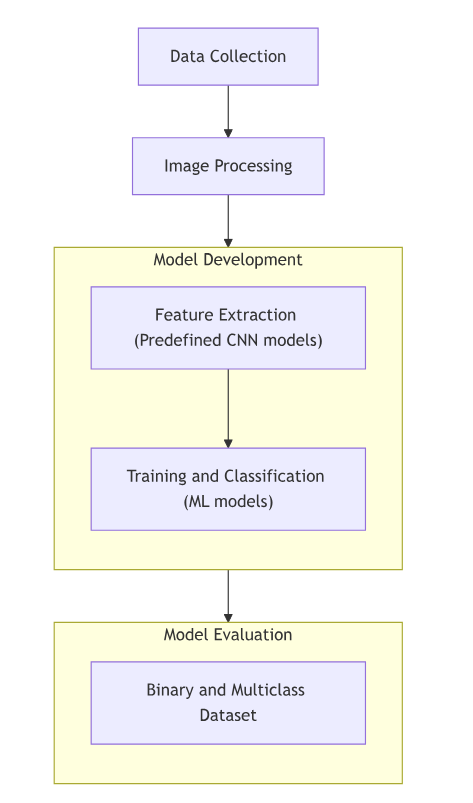
\includegraphics[width=0.385\textwidth]{DOC/flow.png} \caption{Proposed Automated Tomato Quality Grading System} \label{fig:proposed_system} \end{figure}
	
	\section*{3.2 Dataset}
	

\hspace{1cm}The dataset utilized in this research was gathered from agricultural fields in Tamil Nadu, India, with labeling and validation provided by the Department of Horticulture, Tamil Nadu. The dataset was structured to support various classification tasks, with details of the class distribution presented in Table \ref{tab:class_distribution}. Prior to training the models, a series of preprocessing steps were applied. Each image was resized to a standardized 150 x 150 pixels to maintain consistency. Additionally, several data augmentation techniques were employed to diversify the training set and improve the model’s ability to generalize. These techniques included random rotations to introduce variations in image orientation, along with horizontal and vertical flips to simulate different viewpoints. Adjustments to image brightness were made to account for lighting inconsistencies, and random noise was added to simulate real-world conditions, further enhancing the model’s robustness.

\begin{figure}[htbp]\renewcommand\thefigure{3.2} \centering 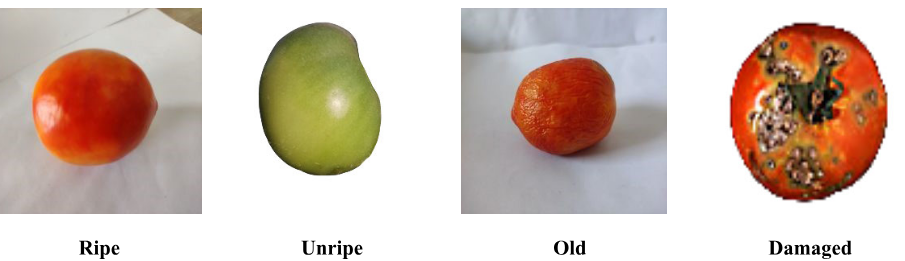
\includegraphics[width=1\textwidth]{DOC/dataset.png} \caption{Sample images from the dataset showcasing the four original classes} \label{fig:dataset} \end{figure}

For classification purposes, the dataset was originally collected as a multiclass dataset, with four categories: ripe, unripe, old, and damaged tomatoes as shown in Figure \ref{fig:dataset}. In the binary classification setup, the classes were redefined to suit market requirements: ripe and unripe tomatoes were categorized as "healthy," while old and damaged tomatoes were grouped as "rejected." This classification structure was chosen based on practical needs in the agricultural and food processing industries, where the distinction between "healthy" and "rejected" tomatoes is crucial for sorting and grading. The distribution of both the binary and multiclass datasets is shown in Table \ref{tab:class_distribution}. The original dataset contained 1,734 images, which increased to 3,466 after augmentation. This increase in dataset size was essential for improving model performance, particularly in achieving better generalization and reducing overfitting during training.
 
	\begin{table}[h]
		\renewcommand\thetable{3.1}
		\centering
		\caption{Class Distribution of the Dataset Before and After Augmentation}
		\renewcommand{\arraystretch}{1.8} % Adjusts the row height
		\begin{tabular}{|c|l|c|c|}
			\hline
			\textbf{S.No} & \textbf{Classes} & \textbf{Original Dataset} & \textbf{After Augmentation} \\ \hline
			1 & Healthy & 932 & 1864 \\ 
			& Rejected & 801 & 1602 \\ \hline
			2 & Ripe & 516 & 1032 \\ 
			& Unripe & 416 & 832 \\ 
			& Old & 435 & 870 \\ 
			& Damaged & 366 & 732 \\ \hline
		\end{tabular}
		\label{tab:class_distribution}
	\end{table}
	
	
	
	\section*{3.3 Feature Extraction Using Pre-trained CNNs}
\hspace{1cm}	In this study, feature extraction was performed using several pre-trained Convolutional Neural Networks (CNNs), including \texttt{ResNet50}, \texttt{InceptionV3}, \texttt{MobileNetV2}, \texttt{DenseNet121}, and \texttt{EfficientNetB0}. These models, pre-trained on large and diverse datasets such as ImageNet, possess the ability to capture a wide range of features from images, enabling the extraction of relevant characteristics essential for classifying tomato quality. The decision to utilize these pre-trained models stems from their exceptional performance in various computer vision tasks, as they have already learned to recognize complex patterns in images, such as edges, textures, and shapes. The feature extraction process, as illustrated in Figure. \ref{fig:feature_extraction}, involves passing input images through the layers of these CNN models. Each layer progressively abstracts the features from low-level information (e.g., edges and textures) to high-level representations (e.g., shapes, objects, and complex patterns). The output from the CNNs consists of feature maps—structured data that encapsulates these learned representations. These feature maps are then stored as tensors, which are multidimensional arrays that hold the extracted features and serve as input for the next stages of the classification pipeline.
	

	
	\begin{figure}[h]
		\renewcommand\thefigure{3.3}
		\centering
		\resizebox{0.9\textwidth}{!}{ % Resize to 80% of the text width, maintaining aspect ratio
			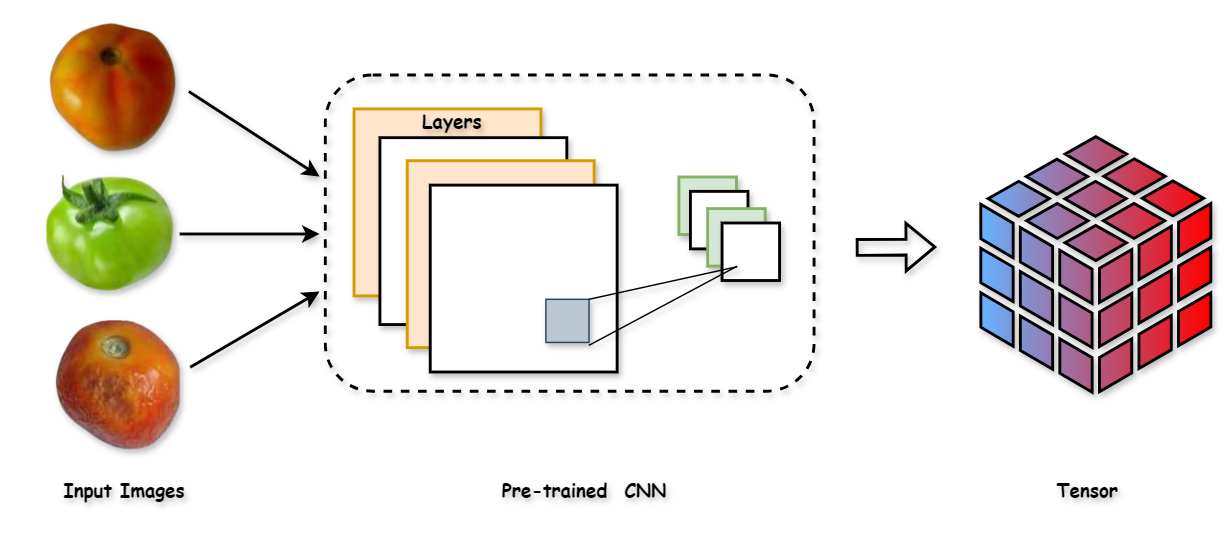
\includegraphics{DOC/FE.png} % Replace with your figure file
		}
		\caption{Feature Extraction Process using Pre-trained CNN Models}
		\label{fig:feature_extraction}
	\end{figure}
	
\hspace{1cm}	To improve the efficiency and accuracy of the tomato classification system, several pre-trained convolutional neural network (CNN) models were employed solely for feature extraction. The models considered in this research included \texttt{ResNet50}\cite{ref8}, \texttt{InceptionV3}\cite{ref9}, \texttt{MobileNetV2}\cite{ref10}, \texttt{DenseNet121}\cite{ref11}, and \texttt{EfficientNetB0}\cite{ref12}. These models, pre-trained on the ImageNet dataset, were selected for their ability to extract high-level features from images efficiently. Each model offers unique architectural innovations that make them suitable for extracting robust and diverse features. \texttt{ResNet50} utilizes residual connections to address the vanishing gradient problem, enabling the extraction of deep hierarchical features. \texttt{InceptionV3} captures features at multiple scales using inception modules. \texttt{MobileNetV2}, optimized for resource-constrained environments, extracts lightweight yet effective features using depthwise separable convolutions. \texttt{DenseNet121} promotes feature reuse through dense connections, resulting in highly detailed feature maps. Finally, \texttt{EfficientNetB0} employs compound scaling to generate compact yet highly informative features. Table \ref{tab:model_features} summarizes the key characteristics of these models, emphasizing their architectural advantages and their suitability for feature extraction.
	
\begin{table}[htbp]
	\renewcommand\thetable{3.2}
	\centering
	\renewcommand{\arraystretch}{2} % Adjust line spacing
	\caption{Key Features of Pre-trained CNN Models for Feature Extraction}
	\label{tab:model_features}
	\begin{tabular}{|l|c|c|c|}
		\hline
		\textbf{Model}           & \textbf{Input Size} & \textbf{Feature Extraction Strength} \\ \hline
		\text{ResNet50}                          & 224 x 224          & Deep hierarchical features          \\ \hline
		\text{InceptionV3}                     & 299 x 299          & Multi-scale spatial features         \\ \hline
		\text{MobileNetV2}                       & 224 x 224          & Efficient lightweight features       \\ \hline
		\text{DenseNet121}                    & 224 x 224          & Detailed and reusable features       \\ \hline
		\text{EfficientNetB0}                    & 224 x 224          & Compact and highly informative       \\ \hline
	\end{tabular}
\end{table}



	
	These pre-trained models served as feature extractors by removing their fully connected layers and leveraging their convolutional layers to generate feature embeddings from the input images. These embeddings were subsequently fed into traditional machine learning classifiers to perform binary and multiclass classification tasks, achieving an optimal balance between computational efficiency and classification accuracy.

	
	\section*{3.4 Classification Algorithms and Methodology}
	
\hspace{1cm}In this study, traditional machine learning classifiers were employed to classify the features extracted by pre-trained CNN models. These classifiers include Support Vector Machine (SVM)\cite{ref18}\cite{ref19}, k-Nearest Neighbors (kNN)\cite{ref20}\cite{ref21},and Decision Trees (DT)\cite{ref22} \cite{ref23}.  The primary objective of utilizing these classifiers was to leverage their ability to efficiently handle both binary and multiclass classification tasks, using the high-dimensional feature sets derived from the CNN models. Each classifier underwent hyperparameter optimization to ensure the best performance on the dataset. The tuning was performed using cross-validation, which enabled a robust evaluation of each model's performance across different subsets of the training data. The goal of hyperparameter optimization was to strike a balance between model complexity and generalization, ensuring that the classifiers perform well without overfitting the data. The SVM classifier was tested with two kernel types: Radial Basis Function (RBF) and Linear, as these are well-suited for handling both linearly separable and non-linearly separable data. The kernel type directly affects the classifier's decision boundary, and selecting the appropriate kernel was crucial for improving classification accuracy. For the kNN algorithm, the number of neighbors was set to 5, based on cross-validation results that suggested it offered the best trade-off between computational cost and accuracy. In the case of the DT algorithm, two configurations were considered for the maximum depth: no limit (None) and a maximum depth of 5. The latter option was chosen to avoid overfitting, which could degrade the model's generalization capability. The hyperparameters used for each classifier are summarized in Table \ref{tab:hyperparameters_classifiers}, which outlines the different configurations tested during the tuning process. These configurations were selected after evaluating various combinations and were chosen based on their impact on classifier performance. This process of fine-tuning and optimizing hyperparameters helped to improve the model's ability to accurately classify tomatoes into their respective categories, enhancing the overall system's performance for both binary and multiclass classification tasks.

	
\begin{table}[h]
	\renewcommand\thetable{3.3}
	\centering
	\caption{Hyperparameters for Traditional Machine Learning Classifiers}
	\renewcommand{\arraystretch}{2.5} % Adjust row height
	\begin{tabular}{|c|l|l|}
		\hline
		\textbf{Classifier} & \textbf{Hyperparameters} & \textbf{Values} \\ \hline
		SupportVectorClassifier & Kernel & rbf, linear \\ \hline
		KNeighborsClassifier & Number of Neighbors & 3, 5 \\ \hline
		DecisionTreeClassifier & Max Depth & None, 3, 5 \\ \hline
		
	\end{tabular}
	\label{tab:hyperparameters_classifiers}
\end{table}



\section*{3.5 Performance Metrics}

\hspace{1cm}The performance of the model is evaluated using several metrics that help assess its effectiveness in classification tasks. These metrics include True Positive (TP), which represents the number of correctly predicted positive cases; True Negative (TN), which corresponds to correctly predicted negative cases; False Positive (FP), which refers to incorrectly predicted positive cases; and False Negative (FN), which denotes incorrectly predicted negative cases.

\subsubsection*{ Accuracy}
\[
\text{Accuracy} = \frac{TP + TN}{TP + TN + FP + FN}
\]
Accuracy represents the proportion of correctly predicted instances out of the total instances. It provides a general measure of the model’s performance, but it may not be suitable for imbalanced datasets, where one class is more prevalent than the other.

\subsubsection*{ Precision}
\[
\text{Precision} = \frac{TP}{TP + FP}
\]
Precision, also known as positive predictive value, measures the ratio of true positive predictions to the total number of positive predictions made by the model. It reflects how many of the instances predicted as positive are actually positive. High precision indicates that the model is making fewer false positive predictions. Precision is particularly important when the cost of a false positive is high, such as in medical diagnoses or fraud detection.

\subsubsection*{ Recall (Sensitivity)}
\[
\text{Recall} = \frac{TP}{TP + FN}
\]
Recall, also known as sensitivity or true positive rate, measures the model's ability to identify all actual positive cases. It reflects how well the model detects positive instances. High recall is essential when the cost of missing a positive case (false negative) is significant, such as in detecting diseases or identifying critical events.

\subsubsection*{F1 Score}
\[
\text{F1 Score} = 2 \times \frac{\text{Precision} \times \text{Recall}}{\text{Precision} + \text{Recall}}
\]
The F1 Score is the harmonic mean of precision and recall. It provides a balance between the two metrics, especially when there is an uneven class distribution. F1 is a more useful metric when both precision and recall are important, and there is a need to balance false positives and false negatives.

\subsubsection*{Confusion Matrix}

\hspace{1cm}The confusion matrix is a tabular representation of the performance of a classification model. It summarizes the true positives, true negatives, false positives, and false negatives in a structured manner. The confusion matrix provides a deeper insight into the errors made by the model, allowing for the identification of specific areas that require improvement. The general structure of a confusion matrix is illustrated in Figure \ref{fig:Confusion_Matrix}, where part (a) represents the binary confusion matrix and part (b) depicts the multiclass confusion matrix.

\begin{figure}[h]
	\renewcommand\thefigure{3.4}
	\centering
	\resizebox{1\textwidth}{!}{ % Resize to 90% of the text width, maintaining aspect ratio
		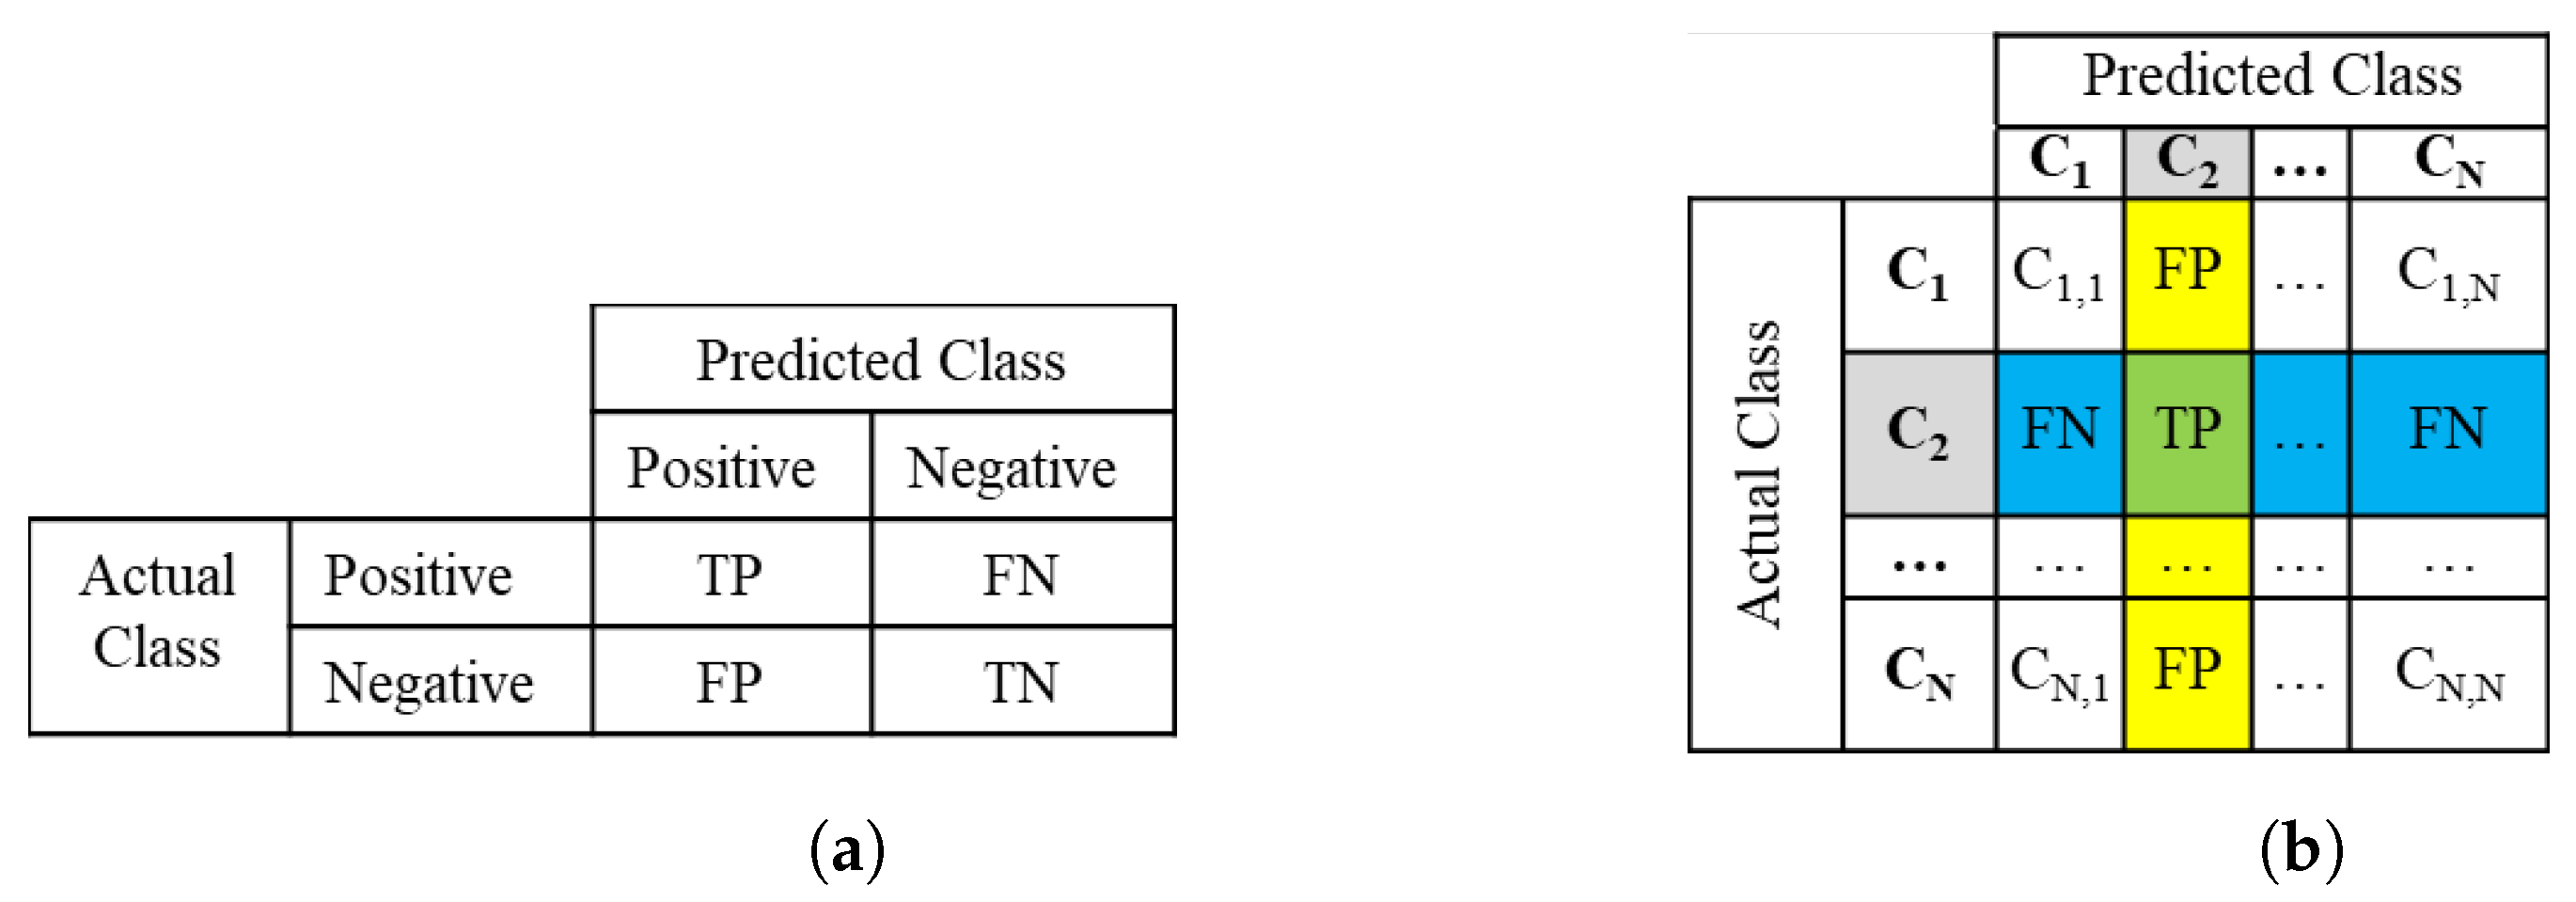
\includegraphics{DOC/cm.png} % Replace with your figure file
	}
	\caption{Illustration of confusion matrices: (a) Binary confusion matrix; (b) Multiclass confusion matrix.}
	\label{fig:Confusion_Matrix}
\end{figure}



    \newpage
	\begin{center}
	\textbf{\Large CHAPTER 4}\\[0.5cm]
	\textbf{\Large  IMPLEMENTATION AND RESULTS}
\end{center}


\section*{4.1 System Architecture}

\hspace{1cm}The system architecture of the proposed automated tomato quality grading and sorting system is designed to seamlessly integrate various components, ensuring real-time performance and high classification accuracy. The architecture comprises multiple stages, each focusing on a specific task, such as image acquisition, feature extraction, classification, and decision-making. The overall workflow is as follows:

\begin{itemize}
	\item \textbf{Image Acquisition}: The first step involves capturing high-quality images of tomatoes using cameras positioned on the production line. These images are fed into the system for further processing.
	
	\item \textbf{Preprocessing and Augmentation}: The acquired images undergo preprocessing steps such as resizing, normalization, and data augmentation (rotation, flipping, brightness adjustment, etc.) to enhance the diversity of the dataset and improve model generalization.
	
	\item \textbf{Feature Extraction}: Pre-trained Convolutional Neural Networks (CNNs) are employed to extract relevant features from the preprocessed images. The extracted features are then passed to traditional machine learning classifiers for classification tasks.
	
	\item \textbf{Classification}: The features extracted from the images are classified using algorithms like Support Vector Machines (SVM), k-Nearest Neighbors (kNN), and Decision Trees (DT) to determine the quality of the tomatoes. Both binary and multiclass classification tasks are handled in this stage.
	
	\item \textbf{Decision and Grading}: Based on the classification results, the system categorizes tomatoes as "healthy" or "rejected" (binary classification) or assigns them to one of the four categories: ripe, unripe, old, or damaged (multiclass classification). The system can then trigger the appropriate action, such as sorting the tomatoes or sending an alert.
\end{itemize}

The architecture ensures that the system is scalable, flexible, and robust enough to handle variations in tomato quality while maintaining high throughput and low error rates.

\begin{figure}[h]
	\renewcommand\thefigure{4.1}
	\centering
	\resizebox{0.8\textwidth}{!}{ 
		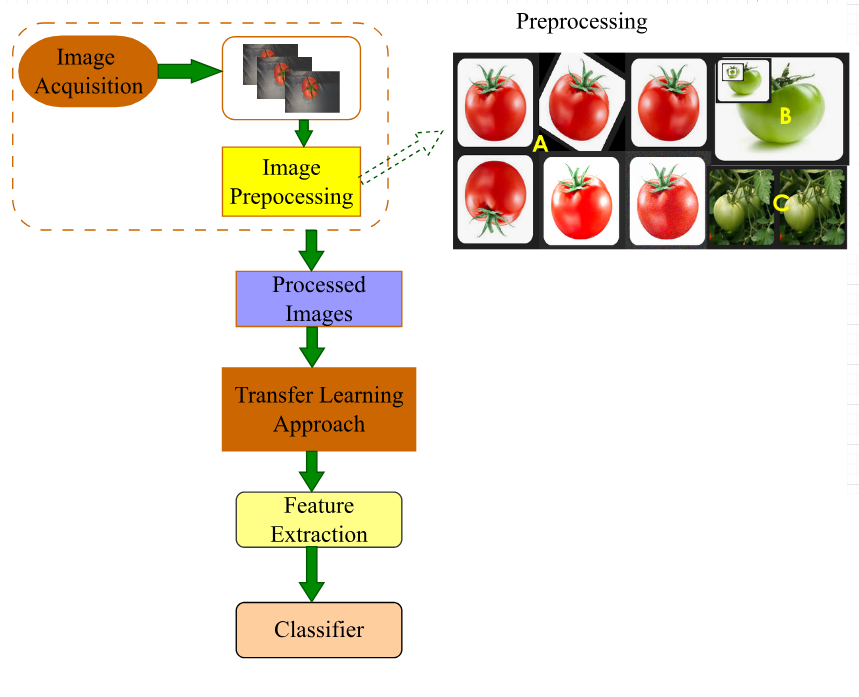
\includegraphics{DOC/artt.png} 
	}
	\caption{System Architecture of the Automated Tomato Quality Grading System.}
	\label{fig:System_Architecture}
\end{figure}

\section*{4.2 Implementation Setup}

\hspace{1cm}The implementation of the automated tomato quality grading and sorting system leverages a high-performance on-premise server configuration to ensure seamless operation and real-time processing capabilities. The server runs on the Ubuntu 22.04.5 LTS operating system and is hosted on a Dell PowerEdge R740 machine, which features an Intel Xeon Gold 6140 processor with 36 cores and an NVIDIA Tesla V100 GPU for accelerated deep learning computations. The system is equipped with 256 GB of RAM and a 2.54 TiB SSD, providing ample resources for handling large-scale image processing and deep learning workflows. Additional features such as a 1600x900 resolution and the zsh 5.8.1 shell further enhance the operational environment. The detailed server specifications are summarized in Table~\ref{tab:server_config}.
\begin{table}[h]
	\renewcommand\thetable{4.1}
	\centering
	\caption{On-Premise Server Specifications}
	\label{tab:server_config}
	\renewcommand{\arraystretch}{1.8}
	\begin{tabular}{|l|l|}
		\hline
		\textbf{Parameter}        & \textbf{Specification}            \\ \hline
		Operating System          & Ubuntu 22.04.5 LTS x86\_64        \\ \hline
		Host Machine              & Dell PowerEdge R740               \\ \hline
		Kernel Version            & 5.15.0-126-generic                \\ \hline
		Shell                     & zsh 5.8.1                         \\ \hline
		Resolution                & 1600x900                          \\ \hline
		CPU                       & Intel Xeon Gold 6140 (36 cores) @ 2.3GHz \\ \hline
		GPU                       & NVIDIA Tesla V100 PCIe 16GB       \\ \hline
		RAM                    & 256        \\ \hline
		SSD                    & 2.54TiB        \\ \hline
	\end{tabular}
\end{table}

\section*{4.3 Feature Extraction Results}

\hspace{1cm}The process of feature extraction from images utilizes pre-trained deep learning models to efficiently derive meaningful representations from the data. This method involves selecting a suitable pre-trained model, such as \texttt{ResNet50}, \texttt{InceptionV3}, \texttt{MobileNetV2}, \texttt{DenseNet121}, or \texttt{EfficientNetB0}, to process the dataset. The input images are resized to a standard dimension of $150 \times 150$ to ensure compatibility with the model architecture. The dataset, organized in a specified directory, is processed in batches, with a default size of 32 images per batch. The features extracted from the images, along with their corresponding labels, are saved as tensors in a designated directory for subsequent use. This approach leverages transfer learning, which eliminates the need for training a model from scratch, thus significantly reducing computational requirements and time. The extracted features can then be utilized for further analysis or as input to traditional machine learning classifiers, enhancing the efficiency and accuracy of downstream tasks.
	
\begin{lstlisting}[language=Python, caption=]
	
	def extract_features(model_name, data_dir, img_height=150, img_width=150, batch_size=32, save_dir='Features'):
	
	"""
	Extract features from images using a pre-trained deep learning model.
	
	Args:
			model_name (str): The name of the pre-trained model.
			data_dir (str): Path to the dir containing the image dataset.
			img_height (int): Height of the input image (default: 150).
			img_width (int): Width of the input image (default: 150).
			batch_size (int): Number of images to process at a time.
			save_dir (str): Dir to save the extracted features and labels.
	
	Saves:
            Extracted features and labels as '.tf' files.
	"""
	
\end{lstlisting}


\section*{4.4 Classification Results for Binary and Multi-Class Tasks}

\hspace{1cm}The classification results for both binary and multi-class tasks highlight the performance of models based on extracted features and traditional machine learning classifiers. Using features from the \texttt{InceptionV3} model, a Support Vector Classifier (SVC) with an RBF kernel achieved an accuracy of 0.94, a precision of 0.95, a recall of 0.91, and an F1-score of 0.93 in the binary classification task. Similarly, the \texttt{DenseNet121} model combined with an SVC using a linear kernel demonstrated strong performance in multi-class classification, achieving an accuracy of 0.96, a precision of 0.90, a recall of 0.95, and an F1-score of 0.93. The implementation details and source code for these experiments can be found in the repository at https://github.com/ragu8/phase1. These results emphasize the effectiveness of combining pre-trained models for feature extraction with traditional classifiers for robust performance in classification tasks.


\section*{4.5 Evaluation Using Performance Metrics}

\hspace{1cm}The evaluation of the models was conducted using key performance metrics, including accuracy, precision, recall, and F1-score. The results for binary classification tasks are summarized in Table \ref{tab:BC}, while the performance of multi-class classification models is detailed in Table \ref{tab:MC}. 

\renewcommand{\arraystretch}{1.9} % Adjust to your preference
\begin{table}[ht]
	\renewcommand\thetable{4.2}
	\centering
	\caption{Binary Model Performance Comparison}
	\begin{tabular}{|l|l|l|l|l|l|l|}
		\hline
		\textbf{ Model}  & \textbf{Parameters} & \textbf{Accuracy} & \textbf{Precision} & \textbf{Recall}  \\ \hline
		InceptionV3 + SVC &   kernel: rbf & 94 & 95 & 91  \\ \hline
		ResNet50 + SVC &   kernel: linear & 83 & 81 & 83  \\ \hline
		EfficientNetB0 + KNN &   n\_neighbors: 5 & 81 & 79 & 81  \\ \hline
		EfficientNetB0 + DT &   max\_depth: 5 & 79 & 0.76 & 80  \\ \hline
		ResNet50 + SVC &   kernel: rbf & 73 & 79 & 57  \\ \hline
	\end{tabular}
	
	\label{tab:BC}
\end{table}

\hspace{1cm}In the binary classification comparison (Table \ref{tab:BC}), the model combining InceptionV3 with an SVC using an RBF kernel achieved the highest accuracy of 94\%, with a precision of 0.95, recall of 0.91, and an F1-score of 0.93. This indicates its superior ability to generalize in distinguishing between the binary classes. On the other hand, ResNet50 paired with an SVC using an RBF kernel showed a lower accuracy of 73\%, with a precision of 0.79 and a recall of 0.57, highlighting its challenges in handling imbalanced or complex data distributions. Figure \ref{fig:Model_Accuracy} (A) visualizes the accuracy comparison for the binary classification task.

\begin{figure}[h]
	\renewcommand\thefigure{4.2}
	\centering
	\resizebox{1\textwidth}{!}{ 
		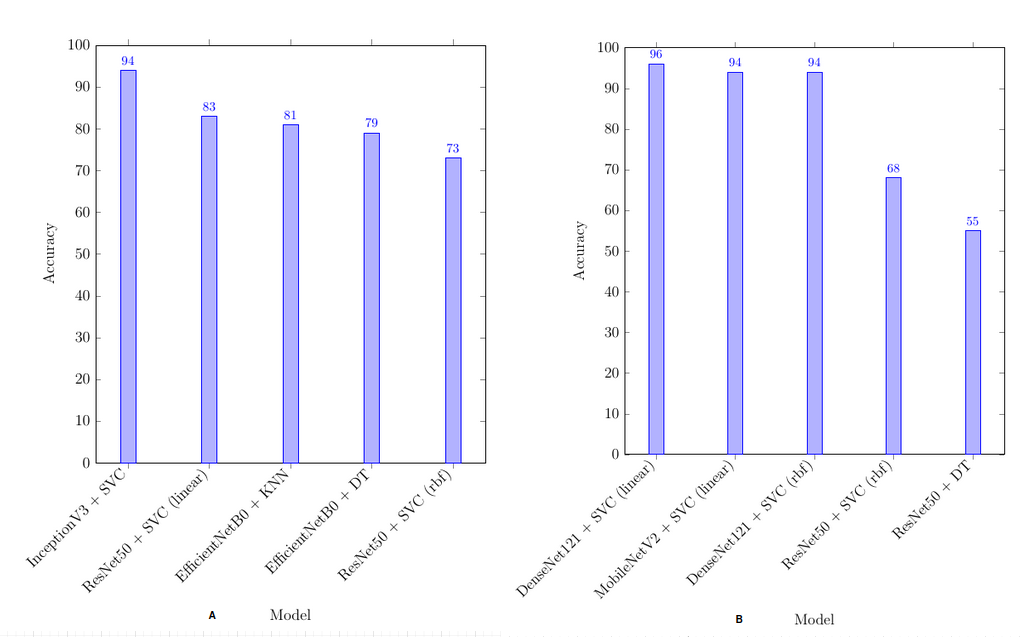
\includegraphics{DOC/acc.png} 
	}
	\caption{Classification Model Accuracy}
	\label{fig:Model_Accuracy}
\end{figure}

For multi-class classification (Table \ref{tab:MC}), the combination of DenseNet121 and SVC (linear kernel) emerged as the top performer, achieving an accuracy of 96\%, precision of 0.91, and recall of 0.96. MobileNetV2 with a linear SVC closely followed with an accuracy of 94\%. 
\renewcommand{\arraystretch}{1.9}
\begin{table}[h!]
	\renewcommand\thetable{4.3}
	\centering
	\caption{Multi-Class Model Performance Comparison}
	\begin{tabular}{|c|c|c|c|c|c|c|}
		\hline
		\textbf{ Model}      & \textbf{Parameters}      & \textbf{Accuracy} & \textbf{Precision} & \textbf{Recall} \\ \hline
		DenseNet121 + SVC & kernel: linear & 96 & 91 & 96 \\ \hline
		MobileNetV2 + SVC & kernel: linear & 94 & 89 & 90 \\ \hline
		DenseNet121 + SVC & kernel: rbf    & 94 & 88 & 94 \\ \hline
		ResNet50+ SVC & kernel: rbf       & 68 & 67 & 56 \\ \hline
		ResNet50 + DT & max\_depth: 5   & 55 & 53 & 36 \\ \hline
	\end{tabular}
	
	\label{tab:MC}
\end{table}
However, the models based on ResNet50 showed relatively lower performance, with the ResNet50 + DT configuration yielding the lowest accuracy of 55\%, precision of 0.53, and recall of 0.36. This indicates potential limitations of ResNet50 for multi-class tasks under the tested configurations. These observations underline the importance of selecting the appropriate feature extractor and classifier combinations based on the complexity and type of the classification task. Figure \ref{fig:Model_Accuracy} (B) illustrates the accuracy for the multi-class classification task.
 
 

The confusion matrices for binary and multi-class tasks, shown in Figure \ref{fig:Conf}, provide insights into model predictions versus actual labels. They highlight correct predictions and misclassifications, aiding in the assessment of model strengths and weaknesses in terms of precision, recall, and accuracy. Figure \ref{fig:Conf} (A) shows the model's ability to distinguish between two classes, while Figure \ref{fig:Conf} (B) evaluates performance across multiple categories.

\begin{figure}[h]
	\renewcommand\thefigure{4.3}
	\centering
	\resizebox{1\textwidth}{!}{ 
		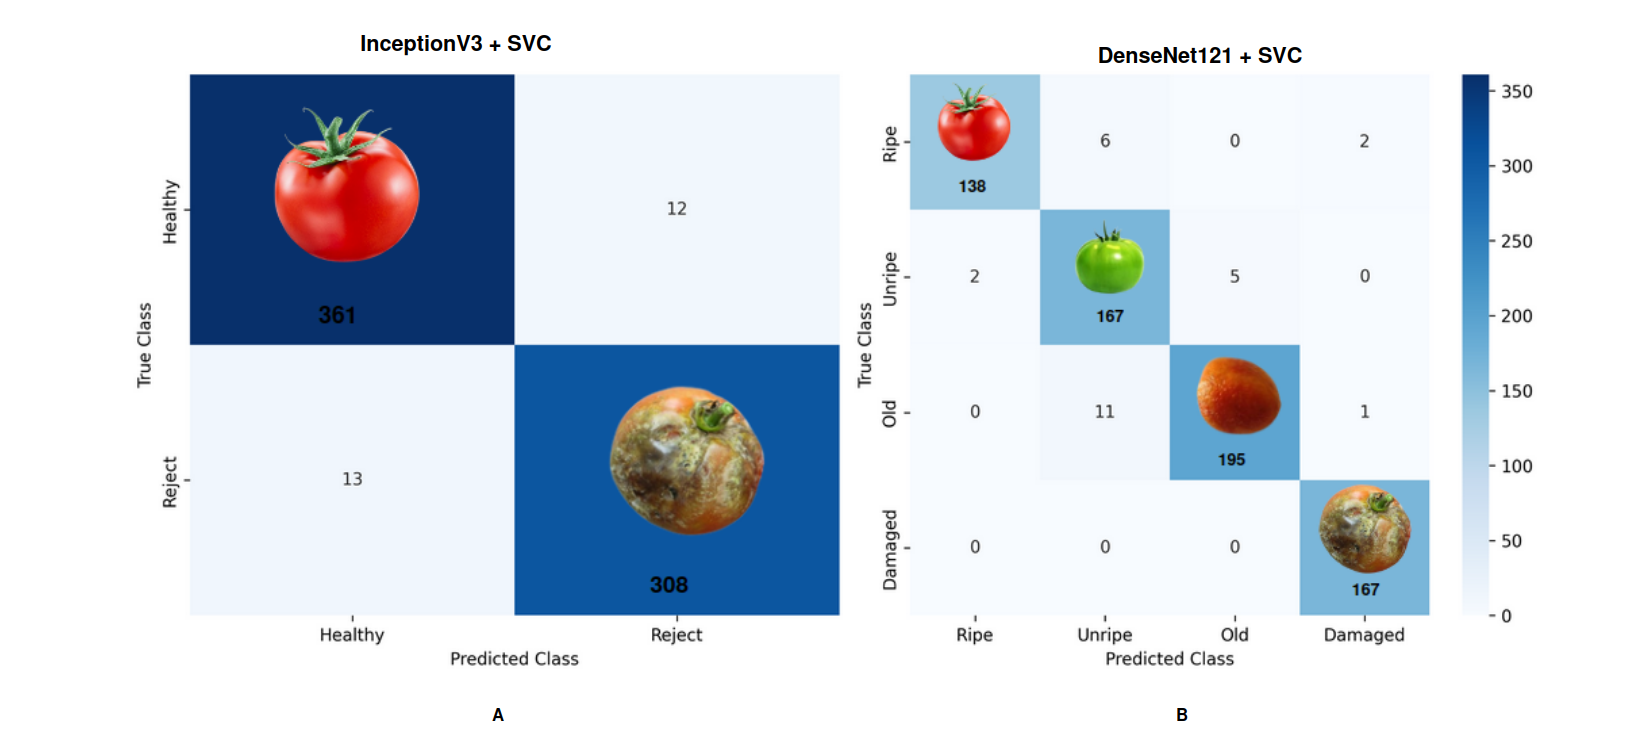
\includegraphics{DOC/CM.png} 
	}
	\caption{Classification Model Confusion Matrix}
	\label{fig:Conf}
\end{figure}

	
\section*{4.6 Discussion on Results}

\hspace{1cm}The classification results demonstrate the effectiveness of using pre-trained deep learning models for feature extraction, combined with traditional machine learning classifiers, in both binary and multi-class classification tasks. The models' performance varies based on the combination of feature extractors and classifiers, which is a critical factor for achieving high accuracy and generalizability. In the \textbf{binary classification} task, the \texttt{InceptionV3 + SVC (RBF kernel)} combination yielded the highest performance, achieving an accuracy of 94\% with excellent precision and recall scores. This suggests that the model is effective at distinguishing between the two classes, even with a relatively simple classifier like SVC. The high precision and recall indicate that the model can both correctly identify positive instances and avoid misclassifying negative instances. However, the performance of the \texttt{ResNet50 + SVC (RBF kernel)} combination was subpar, with an accuracy of just 73\%, precision of 0.79, and recall of 0.57. This lower performance may be due to the difficulty of the ResNet50 model in capturing discriminative features for the binary task, especially when the data distribution is imbalanced or complex. The performance could be improved by fine-tuning the model or exploring alternative classifiers or feature extractors. In the \textbf{multi-class classification} task, the \texttt{DenseNet121 + SVC (linear kernel)} combination performed exceptionally well, with an accuracy of 96\%, precision of 0.91, and recall of 0.96. This indicates that DenseNet121 is well-suited for handling the complexity of multi-class classification, as it effectively extracts features that help the SVC make correct predictions across the different classes. This combination stands out as the most reliable and robust for multi-class tasks, particularly for complex datasets.  On the other hand, \texttt{ResNet50} did not perform as well in multi-class tasks. The \texttt{ResNet50 + DT} combination resulted in the lowest accuracy (55\%), precision (0.53), and recall (0.36), suggesting that this combination may not be ideal for multi-class classification in this specific task. The decision tree classifier may have struggled with the complexity of the feature space or failed to generalize well across the multiple classes. The \texttt{MobileNetV2 + SVC (linear kernel)} also showed strong performance, with an accuracy of 94\%, closely following DenseNet121. This highlights MobileNetV2's potential in scenarios where computational efficiency is crucial, as it provides a good trade-off between accuracy and speed.

The confusion matrices presented in Figure \ref{fig:Conf} further corroborate these findings by visualizing the misclassifications. The models’ ability to correctly predict the classes is evident, but they also highlight areas where improvements can be made, especially in terms of recall for certain classes. For instance, the misclassifications observed in the \texttt{ResNet50 + DT} configuration suggest that this model might be prone to underfitting in multi-class scenarios, which could be addressed by fine-tuning or using a different classifier. Overall, these results highlight the importance of selecting appropriate model configurations based on the task at hand. Pre-trained models like \texttt{InceptionV3} and \texttt{DenseNet121}, combined with traditional machine learning classifiers like \texttt{SVC}, offer a powerful approach to achieve high performance across various classification tasks. However, careful tuning and evaluation of model parameters are necessary to avoid overfitting or underfitting, particularly in more complex multi-class classification scenarios.
	
	
\newpage
\begin{center}
	\textbf{\Large CHAPTER 5}\\[0.5cm]
	\textbf{\Large CONCLUSION AND FUTURE WORK}
\end{center}

\section*{5.1 Conclusion}

\hspace{1cm}In this work, we have successfully developed and evaluated a hybrid approach combining pre-trained deep learning models for feature extraction and traditional machine learning classifiers for both binary and multi-class classification tasks. The results demonstrate that combining state-of-the-art models such as \texttt{InceptionV3}, \texttt{DenseNet121}, and \texttt{MobileNetV2} with classifiers like Support Vector Classifiers (SVC) and K-Nearest Neighbors (KNN) can achieve high accuracy, precision, and recall, outperforming many baseline methods. For binary classification, the combination of \texttt{InceptionV3} and \texttt{SVC (RBF kernel)} emerged as the top performer, while for multi-class tasks, \texttt{DenseNet121} coupled with \texttt{SVC (linear kernel)} achieved outstanding results. These findings highlight the effectiveness of using pre-trained models for feature extraction in conjunction with traditional classifiers, providing a balance between computational efficiency and high classification performance. The work also sheds light on the challenges faced by certain models, such as \texttt{ResNet50} in multi-class classification tasks, where the performance could be further enhanced with better tuning or alternative approaches.

Overall, this research contributes to the growing field of hybrid machine learning models, demonstrating their potential in a variety of classification tasks, and offering insights into model selection and performance evaluation.

\section*{5.2 Future Work}

\hspace{1cm}While the current work has achieved significant results, there are several opportunities for future research and improvement. One promising avenue is the integration of YOLO (You Only Look Once) models for more advanced real-time object detection and classification tasks. YOLO's ability to perform high-speed detection makes it an ideal candidate for applications requiring quick and efficient predictions, such as real-time surveillance or autonomous systems\cite{ref15}\cite{ref16}. Additionally, vision-based large language models (LLMs) can be explored for future work, particularly in the context of multimodal learning, where models can combine visual and textual information to generate more comprehensive and accurate outputs\cite{ref13}\cite{ref14}\cite{ref17}. For example, integrating YOLO models with vision-based LLMs could enhance the understanding and contextualization of visual data, enabling more sophisticated systems capable of both recognizing objects and understanding complex instructions or scenarios. This integration has the potential to elevate tasks such as autonomous navigation, visual question answering, and interactive robotics. Another area for future work involves expanding the dataset and considering more complex architectures, such as Transformers, for both feature extraction and classification. Fine-tuning pre-trained models or adopting new architectures can further improve the generalization ability of the models, especially in more challenging environments or datasets with a larger variety of classes.

In conclusion, the future scope of this research lies in advancing the integration of computer vision, object detection, and multimodal learning models, with potential applications in industries ranging from healthcare to autonomous systems and beyond. By leveraging cutting-edge technologies, future work can push the boundaries of AI, enabling systems that are not only highly accurate but also capable of more complex and nuanced decision-making processes.


\begin{thebibliography}{23}
	
	\bibitem{ref1} A. M. Abdelsalam and M. S. Sayed, ``Real-time defects detection system for orange citrus fruits using multi-spectral imaging,'' in \textit{Proc. IEEE 59th Int. Midwest Symp. Circuits Syst. (MWSCAS)}, Oct. 2016, pp. 1--4.
	
	\bibitem{ref2} N. K. Bahia, R. Rani, A. Kamboj, and D. Kakkar, ``Hybrid feature extraction and machine learning approach for fruits and vegetable classification,'' \textit{Pertanika J. Sci. Technol.}, vol. 27, no. 4, pp. 1693--1708, 2019.
	
	\bibitem{ref3} T. Tao and X. Wei, ``A hybrid CNN–SVM classifier for weed recognition in winter rape field,'' \textit{Plant Methods}, vol. 18, no. 1, p. 29, Dec. 2022.
	
	\bibitem{ref4} Z. Zha, D. Shi, X. Chen, H. Shi, and J. Wu, ``Classification of appearance quality of red grape based on transfer learning of convolution neural network,'' \textit{Tech. Rep.}, 2023.
	
	\bibitem{ref5} S. R. N. Appe, G. Arulselvi, and G. Balaji, ``Tomato ripeness detection and classification using VGG based CNN models,'' \textit{Int. J. Intell. Syst. Appl. Eng.}, vol. 11, no. 1, pp. 296--302, 2023.
	
	\bibitem{ref6} R. G. de Luna, E. P. Dadios, A. A. Bandala, and R. R. P. Vicerra, ``Size classification of tomato fruit using thresholding, machine learning, and deep learning techniques,'' \textit{AGRIVITA J. Agricult. Sci.}, vol. 41, no. 3, pp. 586--596, Oct. 2019.
	
	\bibitem{ref7} H. S. Mputu, A. Abdel-Mawgood, A. Shimada, and M. S. Sayed, ``Tomato quality classification based on transfer learning feature extraction and machine learning algorithm classifiers,'' \textit{IEEE Access}, vol. 12, pp. 8283--8295, 2024, doi: 10.1109/ACCESS.2024.3352745.
	
	\bibitem{ref8} W. Xu, Y.-L. Fu, and D. Zhu, ``ResNet and its application to medical image processing: Research progress and challenges,'' \textit{Comput. Methods Programs Biomed.}, vol. 240, p. 107660, 2023, doi: 10.1016/j.cmpb.2023.107660.
	
	\bibitem{ref9} C. Szegedy, V. Vanhoucke, S. Ioffe, J. Shlens, and Z. Wojna, ``Rethinking the Inception Architecture for Computer Vision,'' in \textit{Proc. IEEE Conf. Comput. Vis. Pattern Recognit. (CVPR)}, 2016, pp. 2818--2826, doi: 10.1109/CVPR.2016.308.
	
	\bibitem{ref10} K. Dong, C. Zhou, Y. Ruan, and Y. Li, ``MobileNetV2 Model for Image Classification,'' in \textit{Proc. Int. Conf. Inf. Technol. Comput. Appl. (ITCA)}, 2020, pp. 476--480, doi: 10.1109/ITCA52113.2020.00106.
	
	\bibitem{ref11} S. G. Siddarth and S. Chokkalingam, ``DenseNet 121 Framework for Automatic Feature Extraction of Diabetic Retinopathy Images,'' in \textit{Proc. Int. Conf. Emerg. Syst. Intell. Comput. (ESIC)}, 2024, pp. 338--342, doi: 10.1109/ESIC60604.2024.10481664.
	
	\bibitem{ref12} V.-T. Hoang and K.-H. Jo, ``Practical Analysis on Architecture of EfficientNet,'' in \textit{Proc. Int. Conf. Hum. Syst. Interact. (HSI)}, 2021, pp. 1--4, doi: 10.1109/HSI52170.2021.9538782.
	
	\bibitem{ref13} W. Lai, T. Zhang, T. L. Lam, and Y. Gao, ``Vision-Language Model-based Physical Reasoning for Robot Liquid Perception,'' in \textit{Proc. 2024 IEEE/RSJ Int. Conf. Intelligent Robots and Systems (IROS)}, 2024, pp. 9652--9659, doi: 10.1109/IROS58592.2024.10801833.
	
	\bibitem{ref14} X. Li, C. Wen, Y. Hu, Z. Yuan, and X. X. Zhu, ``Vision-Language Models in Remote Sensing: Current progress and future trends,'' \textit{IEEE Geoscience and Remote Sensing Magazine}, vol. 12, no. 2, pp. 32--66, 2024, doi: 10.1109/MGRS.2024.3383473.
	
	\bibitem{ref15} J. Redmon, S. Divvala, R. Girshick, and A. Farhadi, ``You Only Look Once: Unified, Real-Time Object Detection,'' in \textit{Proc. 2016 IEEE Conf. Comput. Vis. Pattern Recognit. (CVPR)}, 2016, pp. 779--788, doi: 10.1109/CVPR.2016.91.
	
	\bibitem{ref16} A. K. Sangaiah, F.-N. Yu, Y.-B. Lin, W.-C. Shen, and A. Sharma, ``UAV T-YOLO-Rice: An Enhanced Tiny Yolo Networks for Rice Leaves Diseases Detection in Paddy Agronomy,'' \textit{IEEE Trans. Network Sci. Eng.}, vol. 11, no. 6, pp. 5201--5216, 2024, doi: 10.1109/TNSE.2024.3350640.
	
	\bibitem{ref17} J. Wang, T. Wang, W. Cai, L. Xu, and C. Sun, ``Boosting Efficient Reinforcement Learning for Vision-and-Language Navigation With Open-Sourced LLM,'' \textit{IEEE Robotics and Automation Letters}, vol. 10, no. 1, pp. 612--619, 2025, doi: 10.1109/LRA.2024.3511402.
	
	\bibitem{ref18} S. S. Teja Gontumukkala, Y. S. Varun Godavarthi, B. R. Ravi Teja Gonugunta, R. Subramani, and K. Murali, ``Analysis of Image Classification using SVM,'' in \textit{Proc. 2021 12th Int. Conf. Comput. Commun. Networking Technol. (ICCCNT)}, 2021, pp. 1--6, doi: 10.1109/ICCCNT51525.2021.9579803.
	
	\bibitem{ref19} X. Sun, L. Liu, H. Wang, W. Song, and J. Lu, ``Image classification via support vector machine,'' in \textit{Proc. 2015 4th Int. Conf. Comput. Sci. Network Technol. (ICCSNT)}, 2015, vol. 1, pp. 485--489, doi: 10.1109/ICCSNT.2015.7490795.
	
	\bibitem{ref20} D. Patidar, B. C. Shah, and M. R. Mishra, ``Performance analysis of K Nearest Neighbors image classifier with different wavelet features,'' in \textit{Proc. 2014 Int. Conf. Green Comput. Commun. Electr. Eng. (ICGCCEE)}, 2014, pp. 1--6, doi: 10.1109/ICGCCEE.2014.6922459.
	
	\bibitem{ref21} E. C. Ozan, E. Riabchenko, S. Kiranyaz, and M. Gabbouj, ``A vector quantization based k-NN approach for large-scale image classification,'' in \textit{Proc. 2016 Int. Conf. Image Process. Theory, Tools Appl. (IPTA)}, 2016, pp. 1--6, doi: 10.1109/IPTA.2016.7821010.
	
	\bibitem{ref22} C. Agarwal and A. Sharma, ``Image understanding using decision tree based machine learning,'' in \textit{Proc. 5th Int. Conf. Inf. Technol. Multimedia (ICIMU)}, 2011, pp. 1--8, doi: 10.1109/ICIMU.2011.6122757.
	
	\bibitem{ref23} H. Liu, M. Cocea, and W. Ding, ``Decision tree learning based feature evaluation and selection for image classification,'' in \textit{Proc. 2017 Int. Conf. Mach. Learn. Cybernet. (ICMLC)}, 2017, vol. 2, pp. 569--574, doi: 10.1109/ICMLC.2017.8108975.
	
\end{thebibliography}


\end{document}
